\section{Results} 
To make the simulation results easier to understand we begin by outlining a baseline model with one independent  variable of interest and two covariates split by the different model sets. We then add the different flexibilities one at a time to examine how much each flexibility by itself contributes to the FPP and FPR compared to the baseline model.

\subsection{Model specification}
Looking at the FPP and FPR between the different sets in the baseline model, it is clear that the highest FPP and FPR are obtained in the $x \times z$ and $x + z+ x \times z$ sets (see Figure \ref{fig:mainfigure1}). This is the case when using interaction terms both when the corresponding main effects are present and whey they are not present. When the corresponding main effects are not present and the covariates and the variable of interest are binary and dummy coded, the high FPP and FPR occurs because the interaction term  captures the true effect of the covariates as the dummy coded variable of interest splits the effect into the interaction and the constant. In this case, the FPP for the $x \times z$ set is 82.7\% and 86.9\% for the $x + z+ x \times z$ set. When the variables are continuous and everything else is equal, the FPP for the two sets are 18.8\% and 23.5\%, respectively. With the restriction that main effects must follow interactions, only the $x + z+ x \times z$ set remains because the $x \times z$ set becomes an empty set. In this case, the FPP is 21.1\% for binary variables and 18.1\% for continuous variables. Looking across all sets at the same time, with no restrictions regarding main effects the FPP is 87.2\% when using two binary covariates variables, and 25.5\% when the variables are continuous and with restrictions on main effects the FPP is 21.5\% and 18.8\%, respectively.\\ 
Looking at the FPR, we see that in general the proportion of models with a significant effect is around the expected 5\%  (see red bars in Figure \ref{fig:mainfigure1}). However, in sets with interactions between the variable of interest and covariates with omitted main effects (left hand side of Figure \ref{fig:mainfigure1}), the FPR is above 5\%. For the $x \times z$ set with binary data and without corresponding main effects the FPR is 34.5\%. \\

% plot of main analysis
\begin{figure}[hbt!]
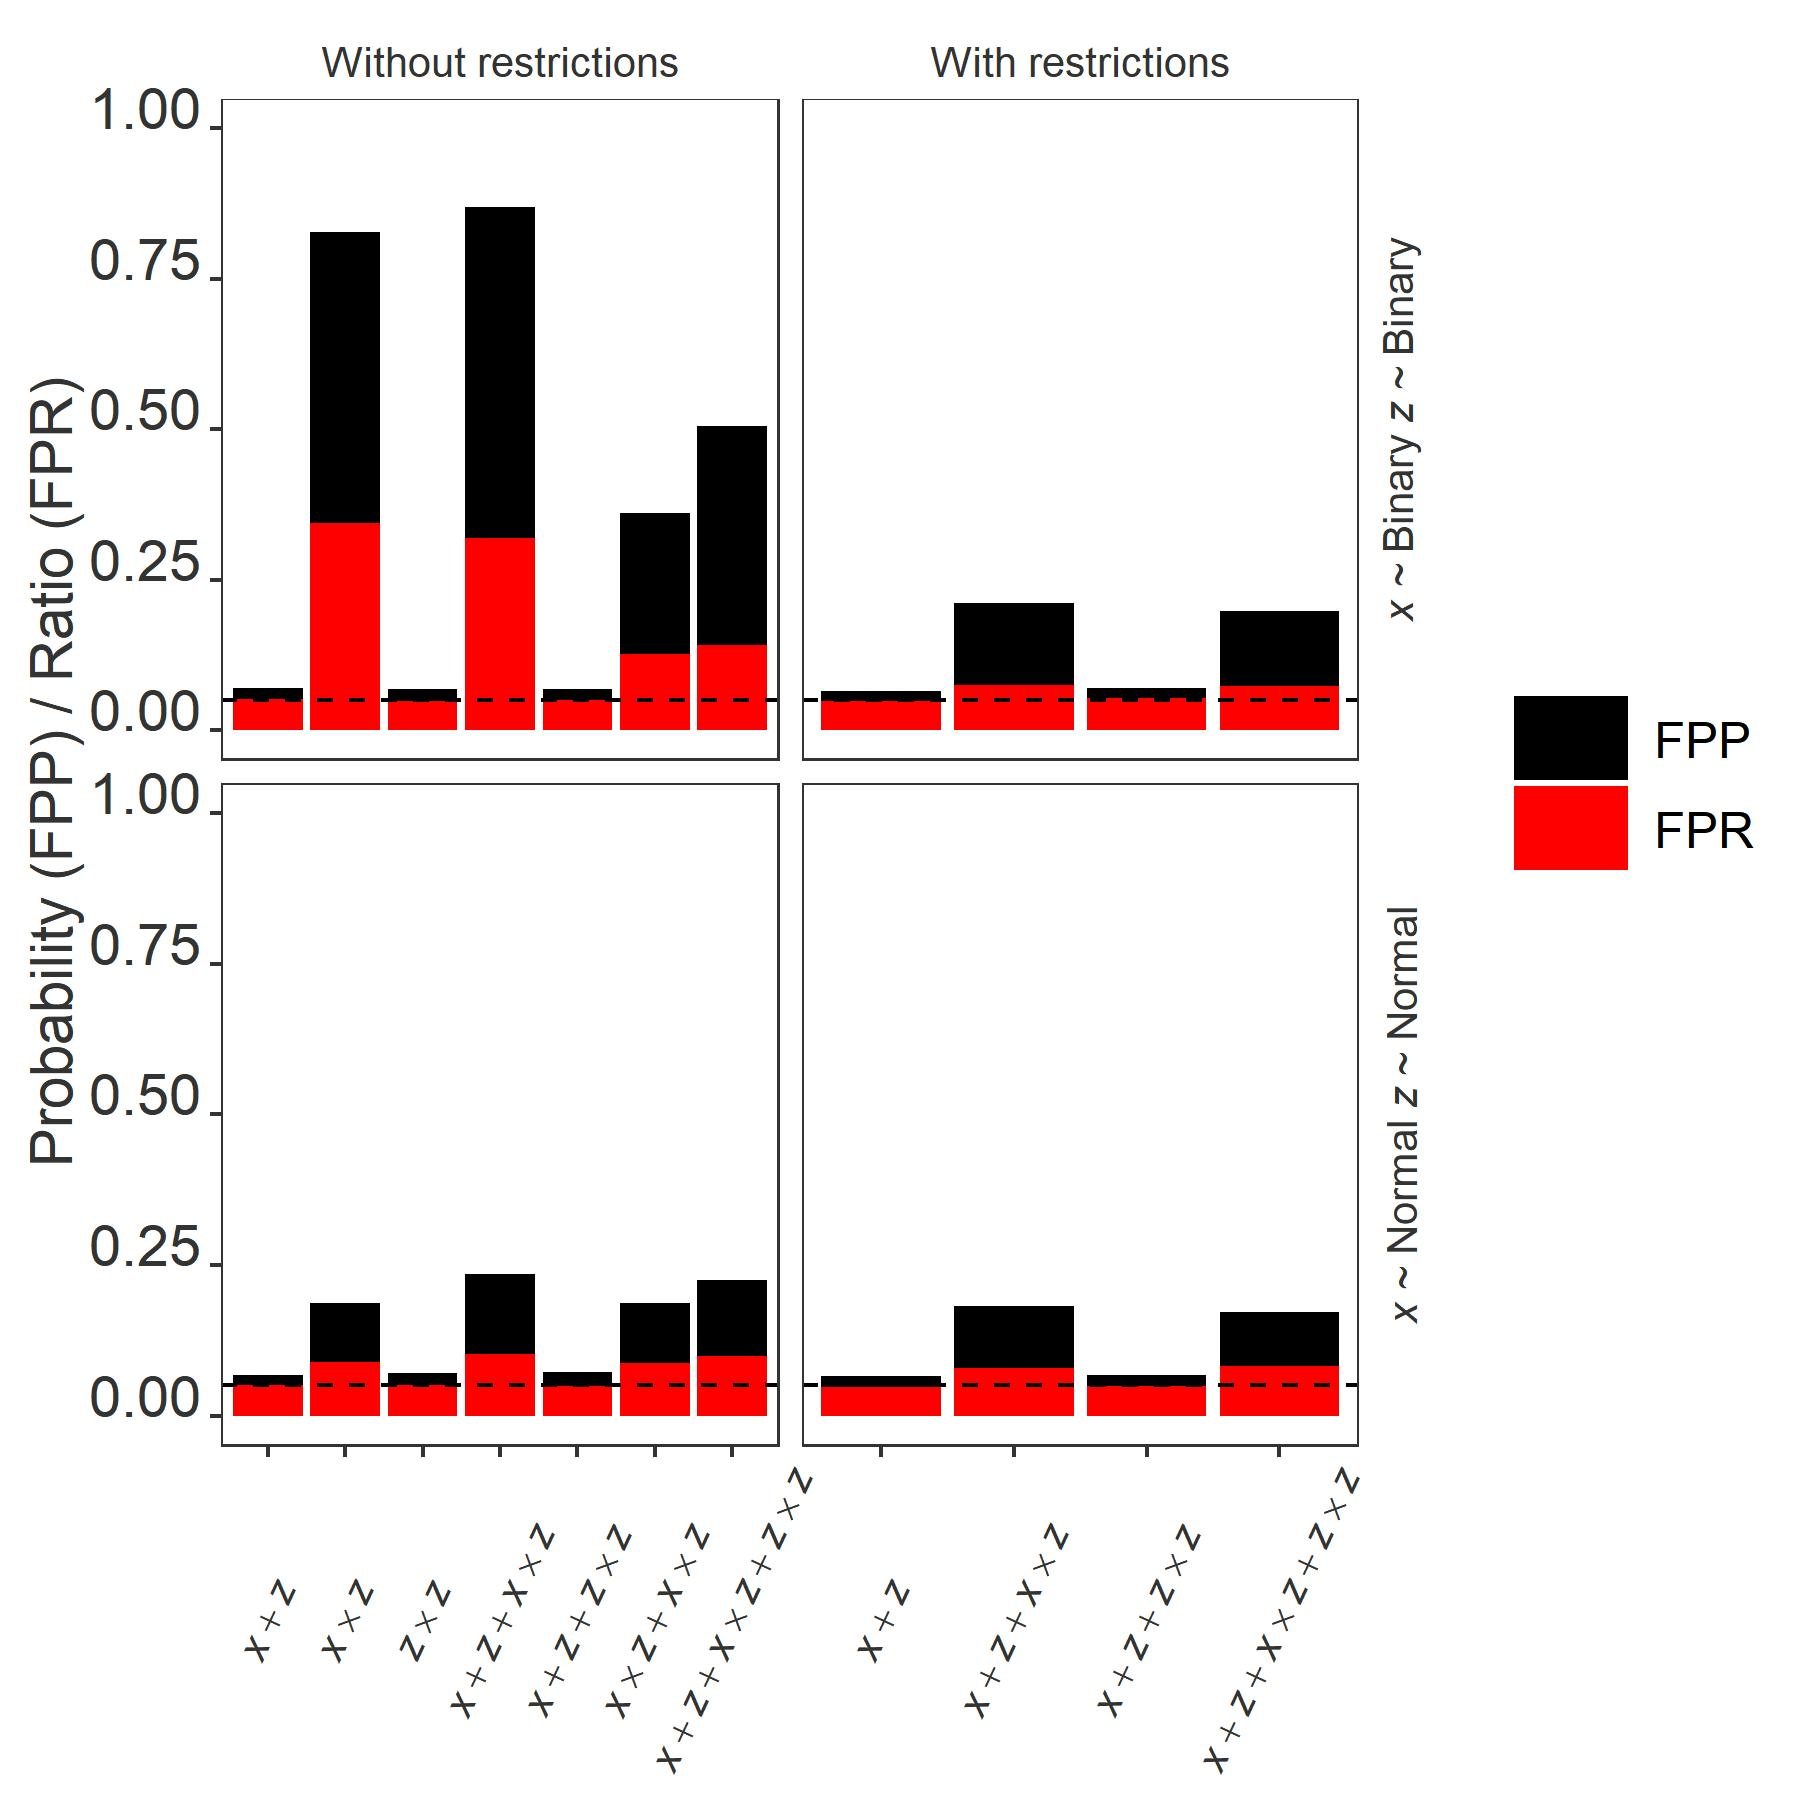
\includegraphics[width=0.6\textwidth]{R/Analysis/Result/Figures/Figure1A.jpeg}
\centering
\caption{The rates of the false-positive probability and false-positive ratio given different model sets, the presence of main effects when having interactions, and different distributions of the variable of interest and covariates. Sample size is set to 200, a correlation between the dependent variable and covariates is \textit{r}=0.2 and we used two covariates. The false-positive probability is shown in black and the false-positive ratio in red. Dashed blacked line indicates 0.05}
\label{fig:mainfigure1}
\end{figure}

\subsection{Number of covariates}
Adding one more covariate to the baseline model to get three in total increases the FPP across all model sets (see Figure \ref{fig:mainfigure2}). The increase is the highest for binary data with no restrictions on main effects to follow interaction terms. Several of the sets with interactions between the variable of interest and covariates reach a FPP just below 100\%. The increase is also evident even when main effects are present when having interactions. In that case, the largest increase in the FPP is in the $x + z+ x \times z + z \times z$ set which increases 14.7 percentage points when the variable of interest and covariates are binary and 13.1 percentage points when the variables are continuous. The FPR also increases for all sets with an interaction between the variable of interest and the covariates although the main increase happens when there is no restriction that the main effect most follow all interactions. 

% plot of main analysis
\begin{figure}[hbt!]
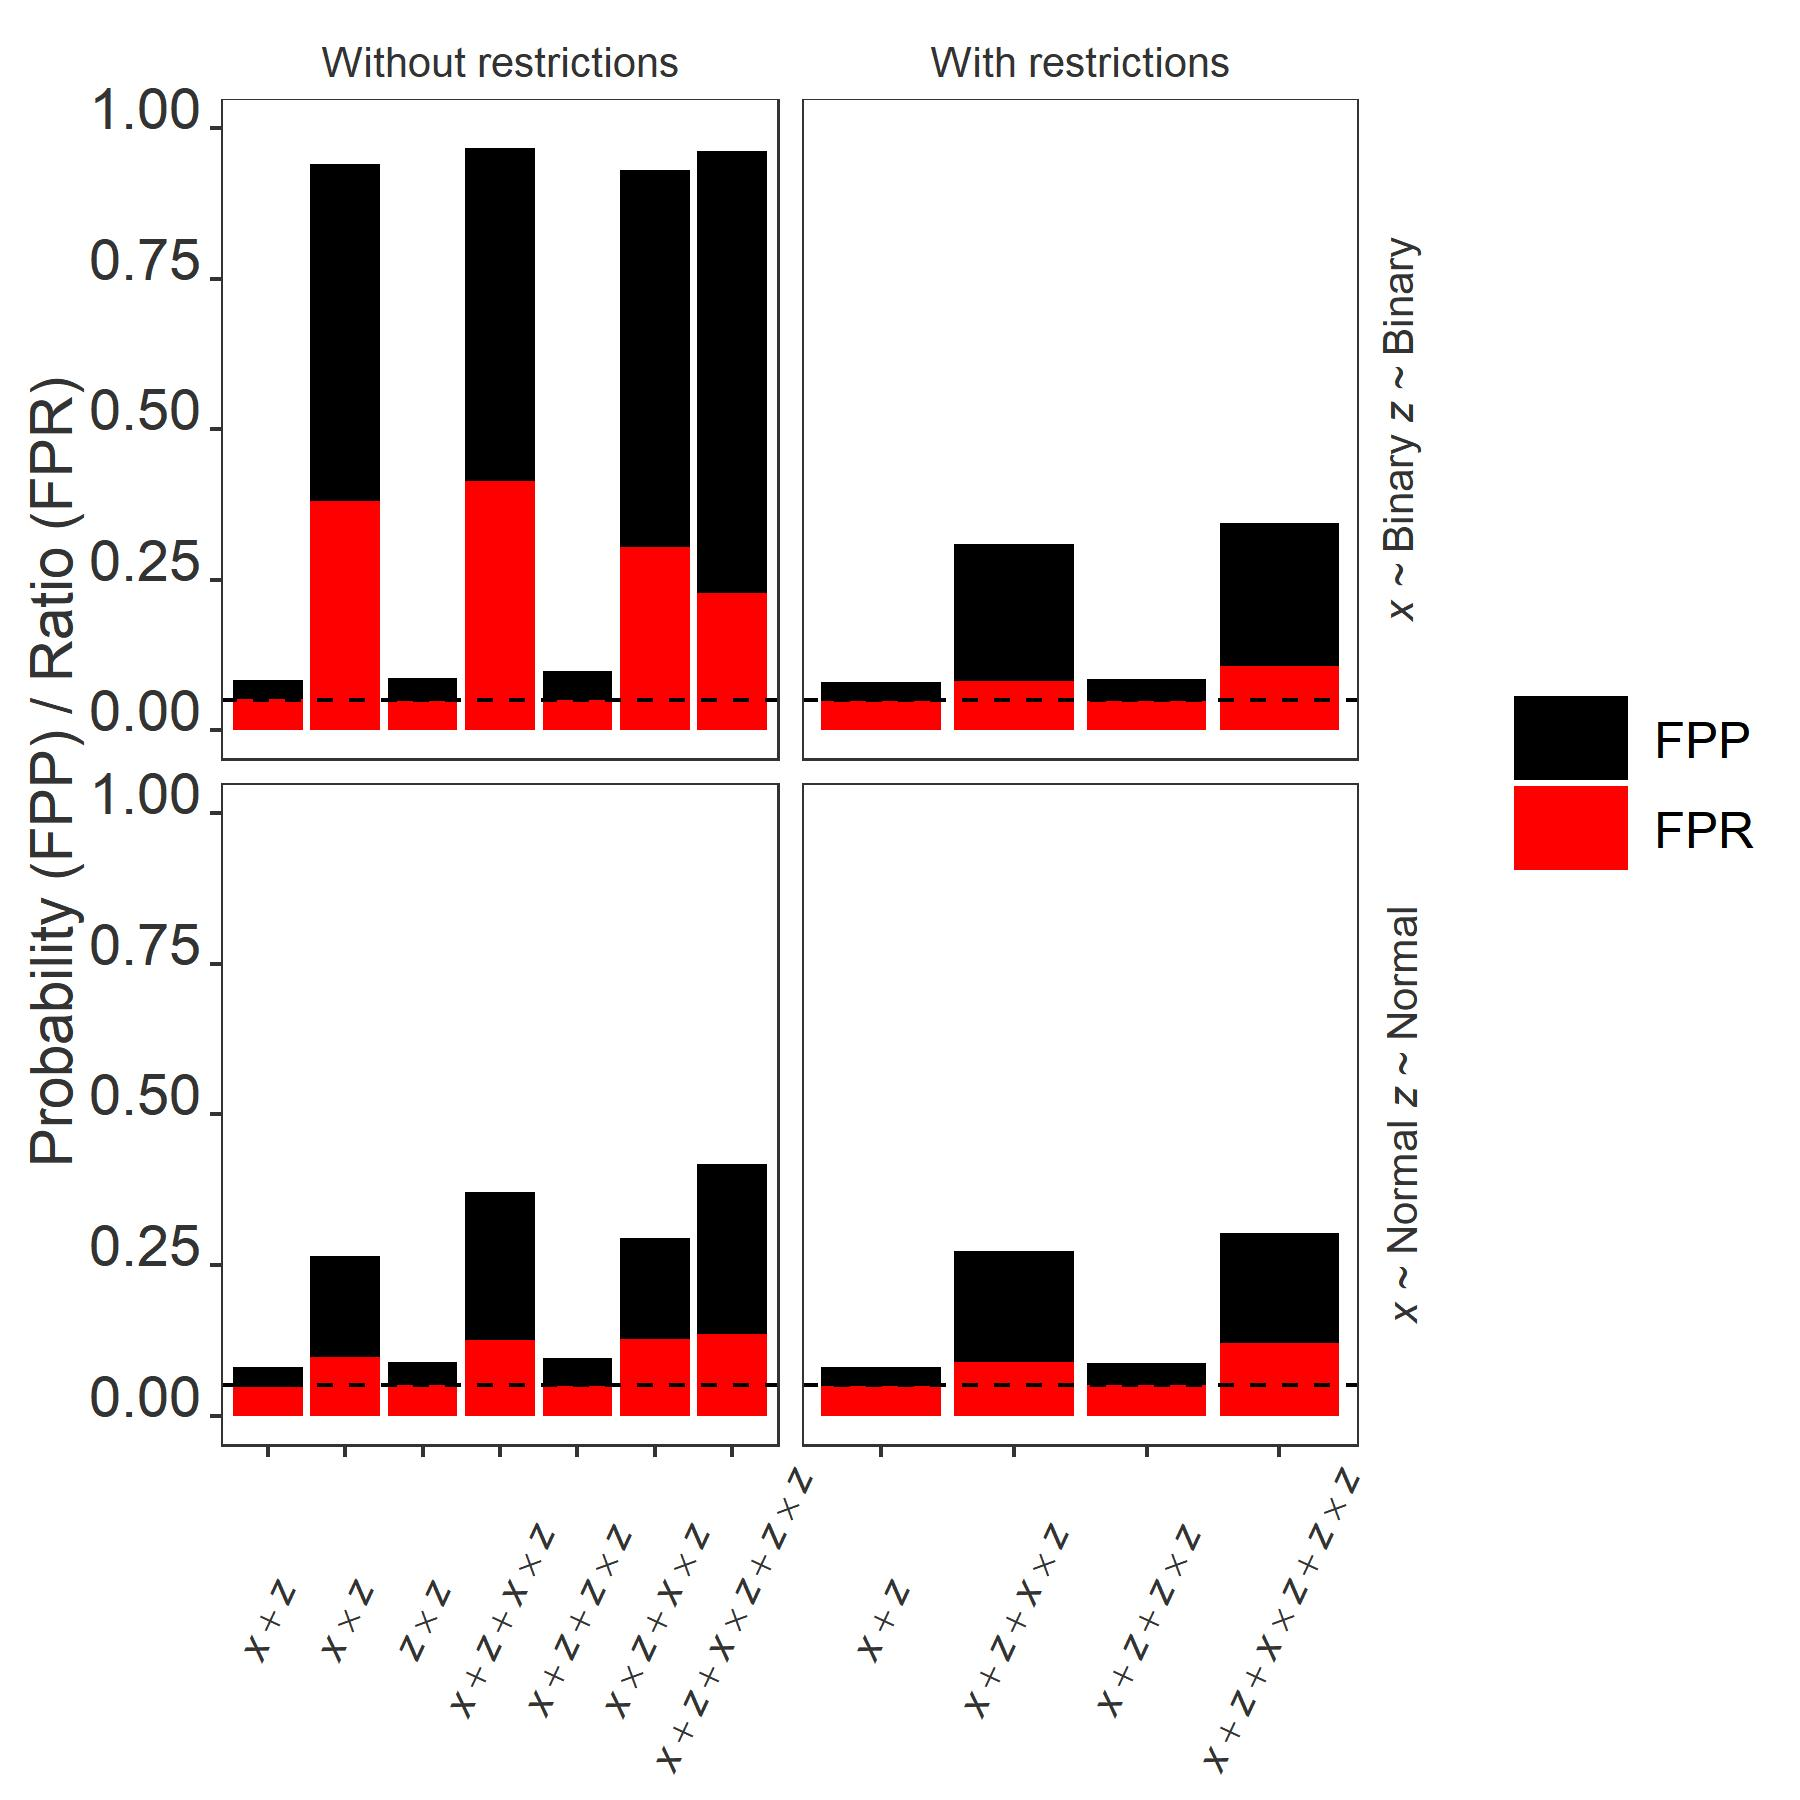
\includegraphics[width=0.6\textwidth]{R/Analysis/Result/Figures/Figure1C.jpeg}
\centering
\caption{The false-positive probability and false-positive ratio when using one more covariate (three in total). Black bars are the false-positive probability and red denotes the false-positive ratio. Dashed blacked line indicates 0.05. The description of the figure is otherwise the same as for Figure \ref{fig:mainfigure1}.}
\label{fig:mainfigure2}
\end{figure}

\subsection{Outlier criteria}
Using the four outlier criteria have different effects depending on the model sets and the data structures (see Figure \ref{fig:mainfigure3}). Overall, the added effect to the FPP ranges between 3.7 and 18.7 percentage points with the largest effects occurring in sets with interactions between the variable of interest and covariates. The smaller added effect for some sets stem from the fact that the FPP is already close to 100\%. Surprisingly, using outlier criteria did not increase the FPR and in some cases even decreased it. 

\begin{figure}[hbt!]
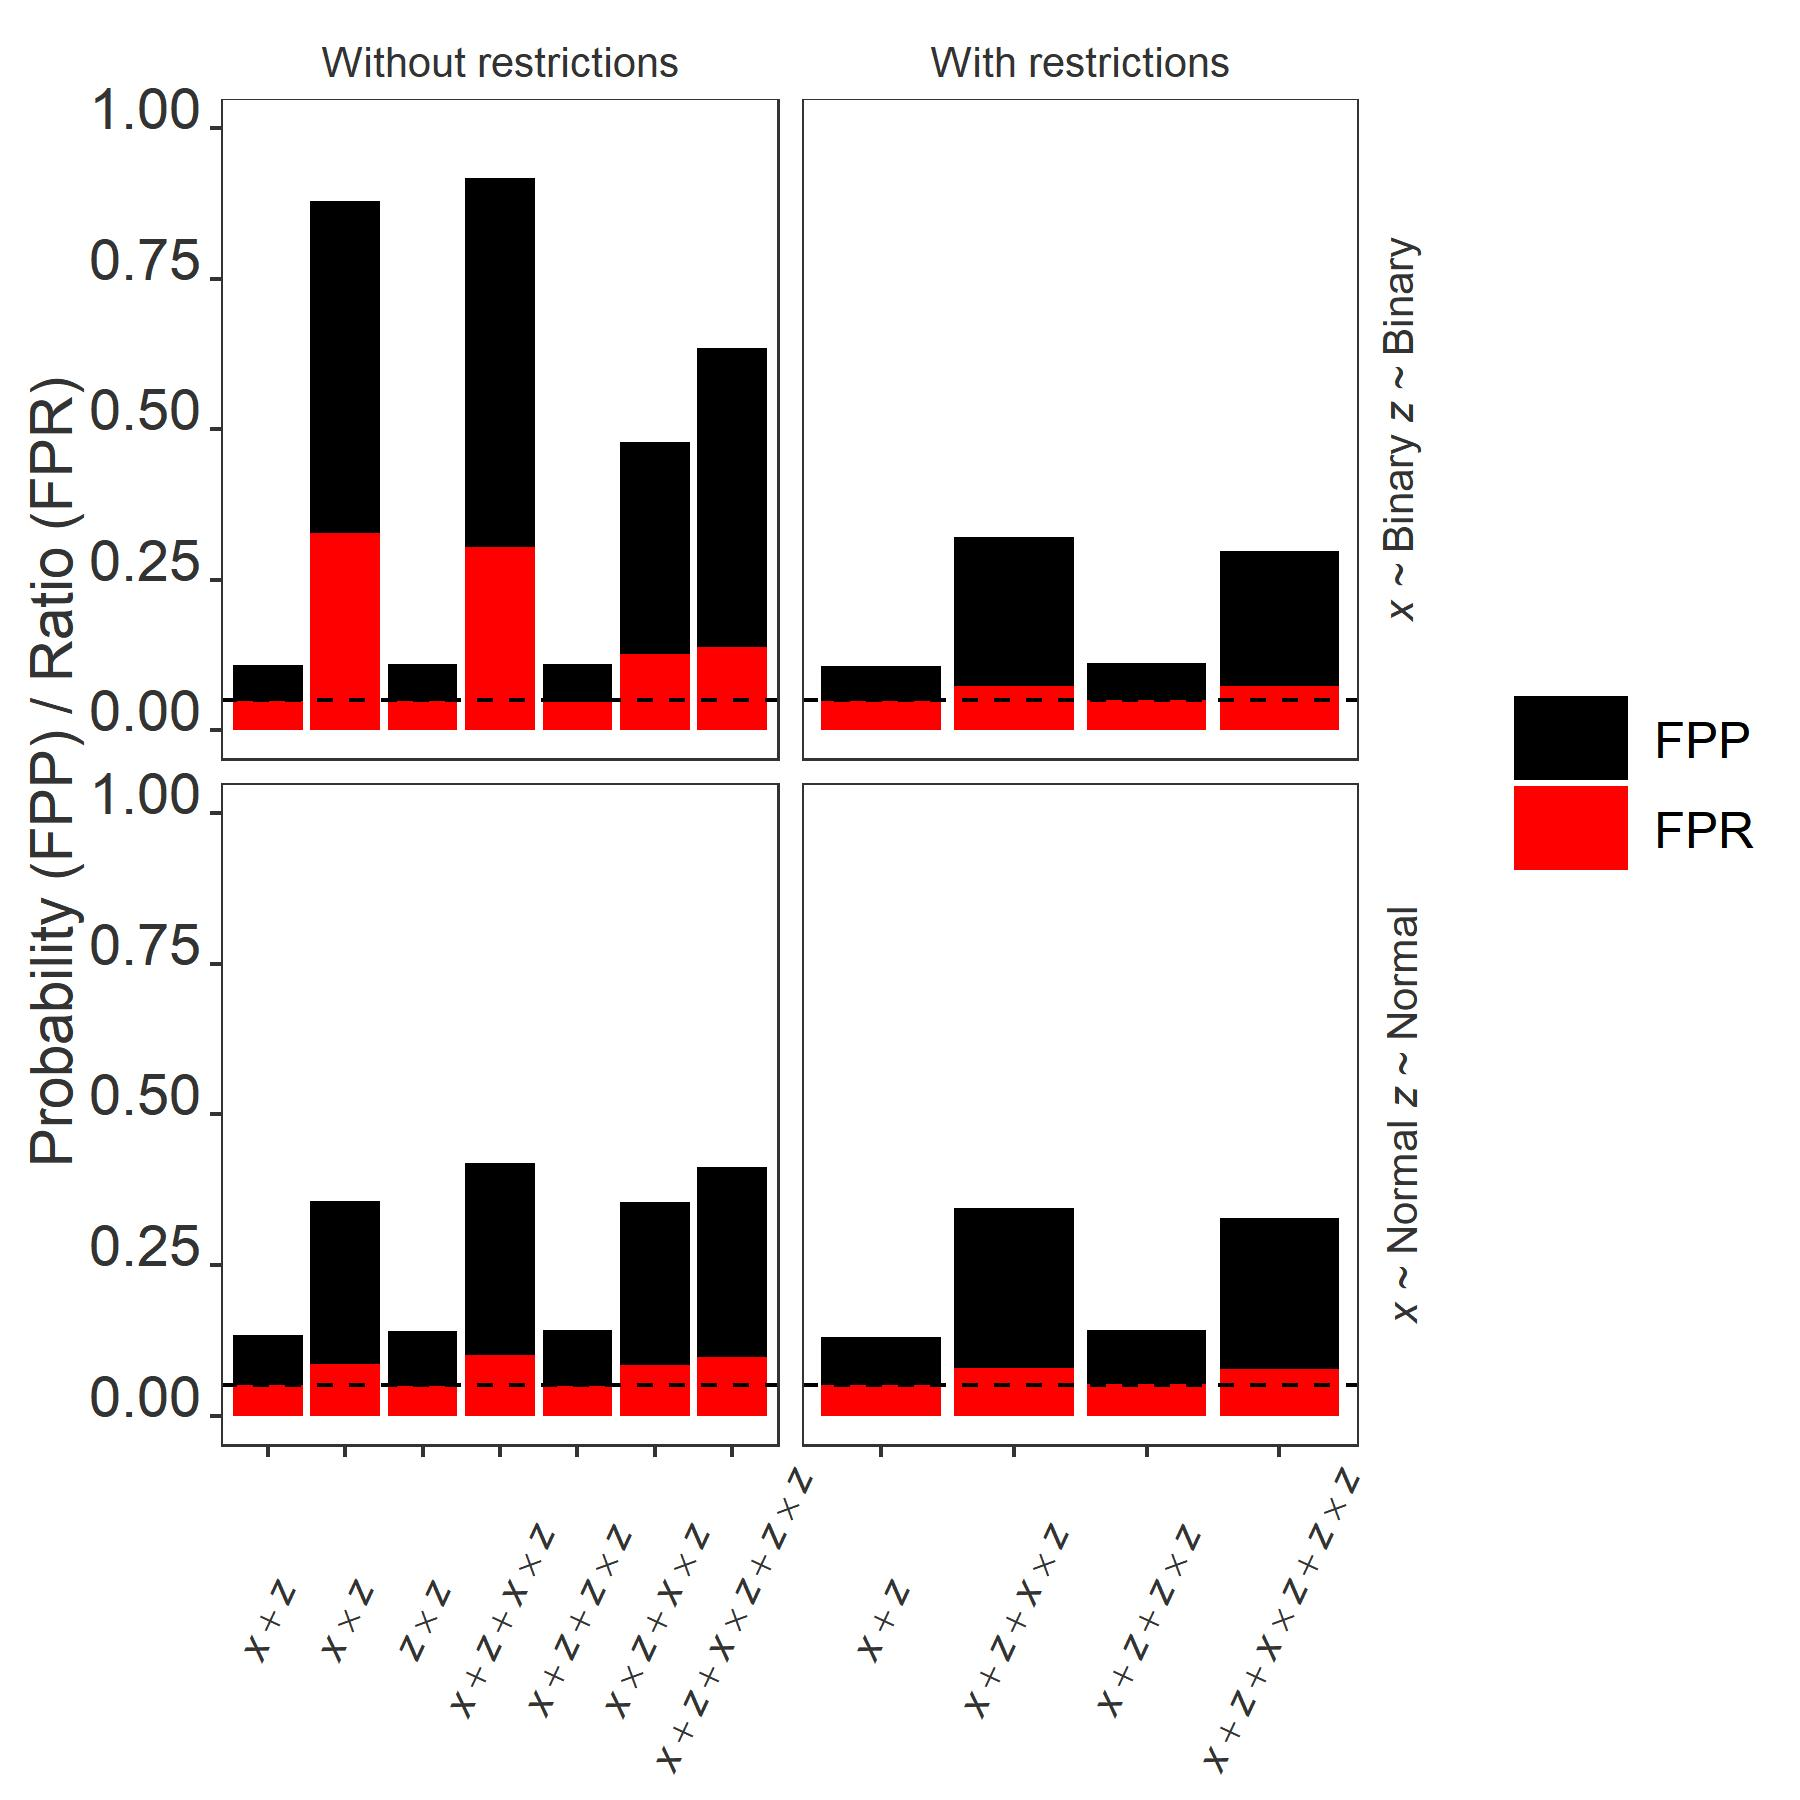
\includegraphics[width=0.6\textwidth]{R/Analysis/Result/Figures/Figure1B.jpeg}
\centering
\caption{The false-positive probability and false-positive ratio hen using multiple outlier criteria. Black bars are the false-positive probability and red denotes the false-positive ratio. Dashed blacked line indicates 0.05. The description of the figure is otherwise the same as for Figure \ref{fig:mainfigure1}.}
\label{fig:mainfigure3}
\end{figure}

\subsection{Multiple dependent variables}
Adding a dependent variable to the baseline model with a correlation of (\textit{r}=0.5) to the other dependent variable and computing the average between the two dependent variables to yield three dependent variables increases the FPP for all model sets. The added effect on FPP ranges from 6.2 to 23.8 percent (see Figure \ref{fig:appfigure3} and Table \ref{tab:apptab6} in Supplementary Material). There was no real changes for the FPR for any set as including extra dependent variables and their average only increased the model set but did nothing to the construction of them (see Figure \ref{fig:appfigure3} Table \ref{tab:apptab6} in Supplementary Material).   

\subsection{Sample size}
Increasing the sample size in the baseline model and thereby improving the precision of the estimates have, in most of the conditions, no effect on either the FPP or FPR. However, in sets with interactions between the variable of interest and covariates where main effects are not included and variables are binary larger sample sizes increase the FPP (See Figure \ref{fig:mainfigure4}). In the $x \times z$ and $x + z+ x \times z$ sets the FPP reaches just below 100\% as the sample size increases to 300. In these sets, the larger sample sizes also lead to increases in the FPR with the largest effect of 41.9\% for the $x \times z$ set.  


\begin{figure}[hbt!]
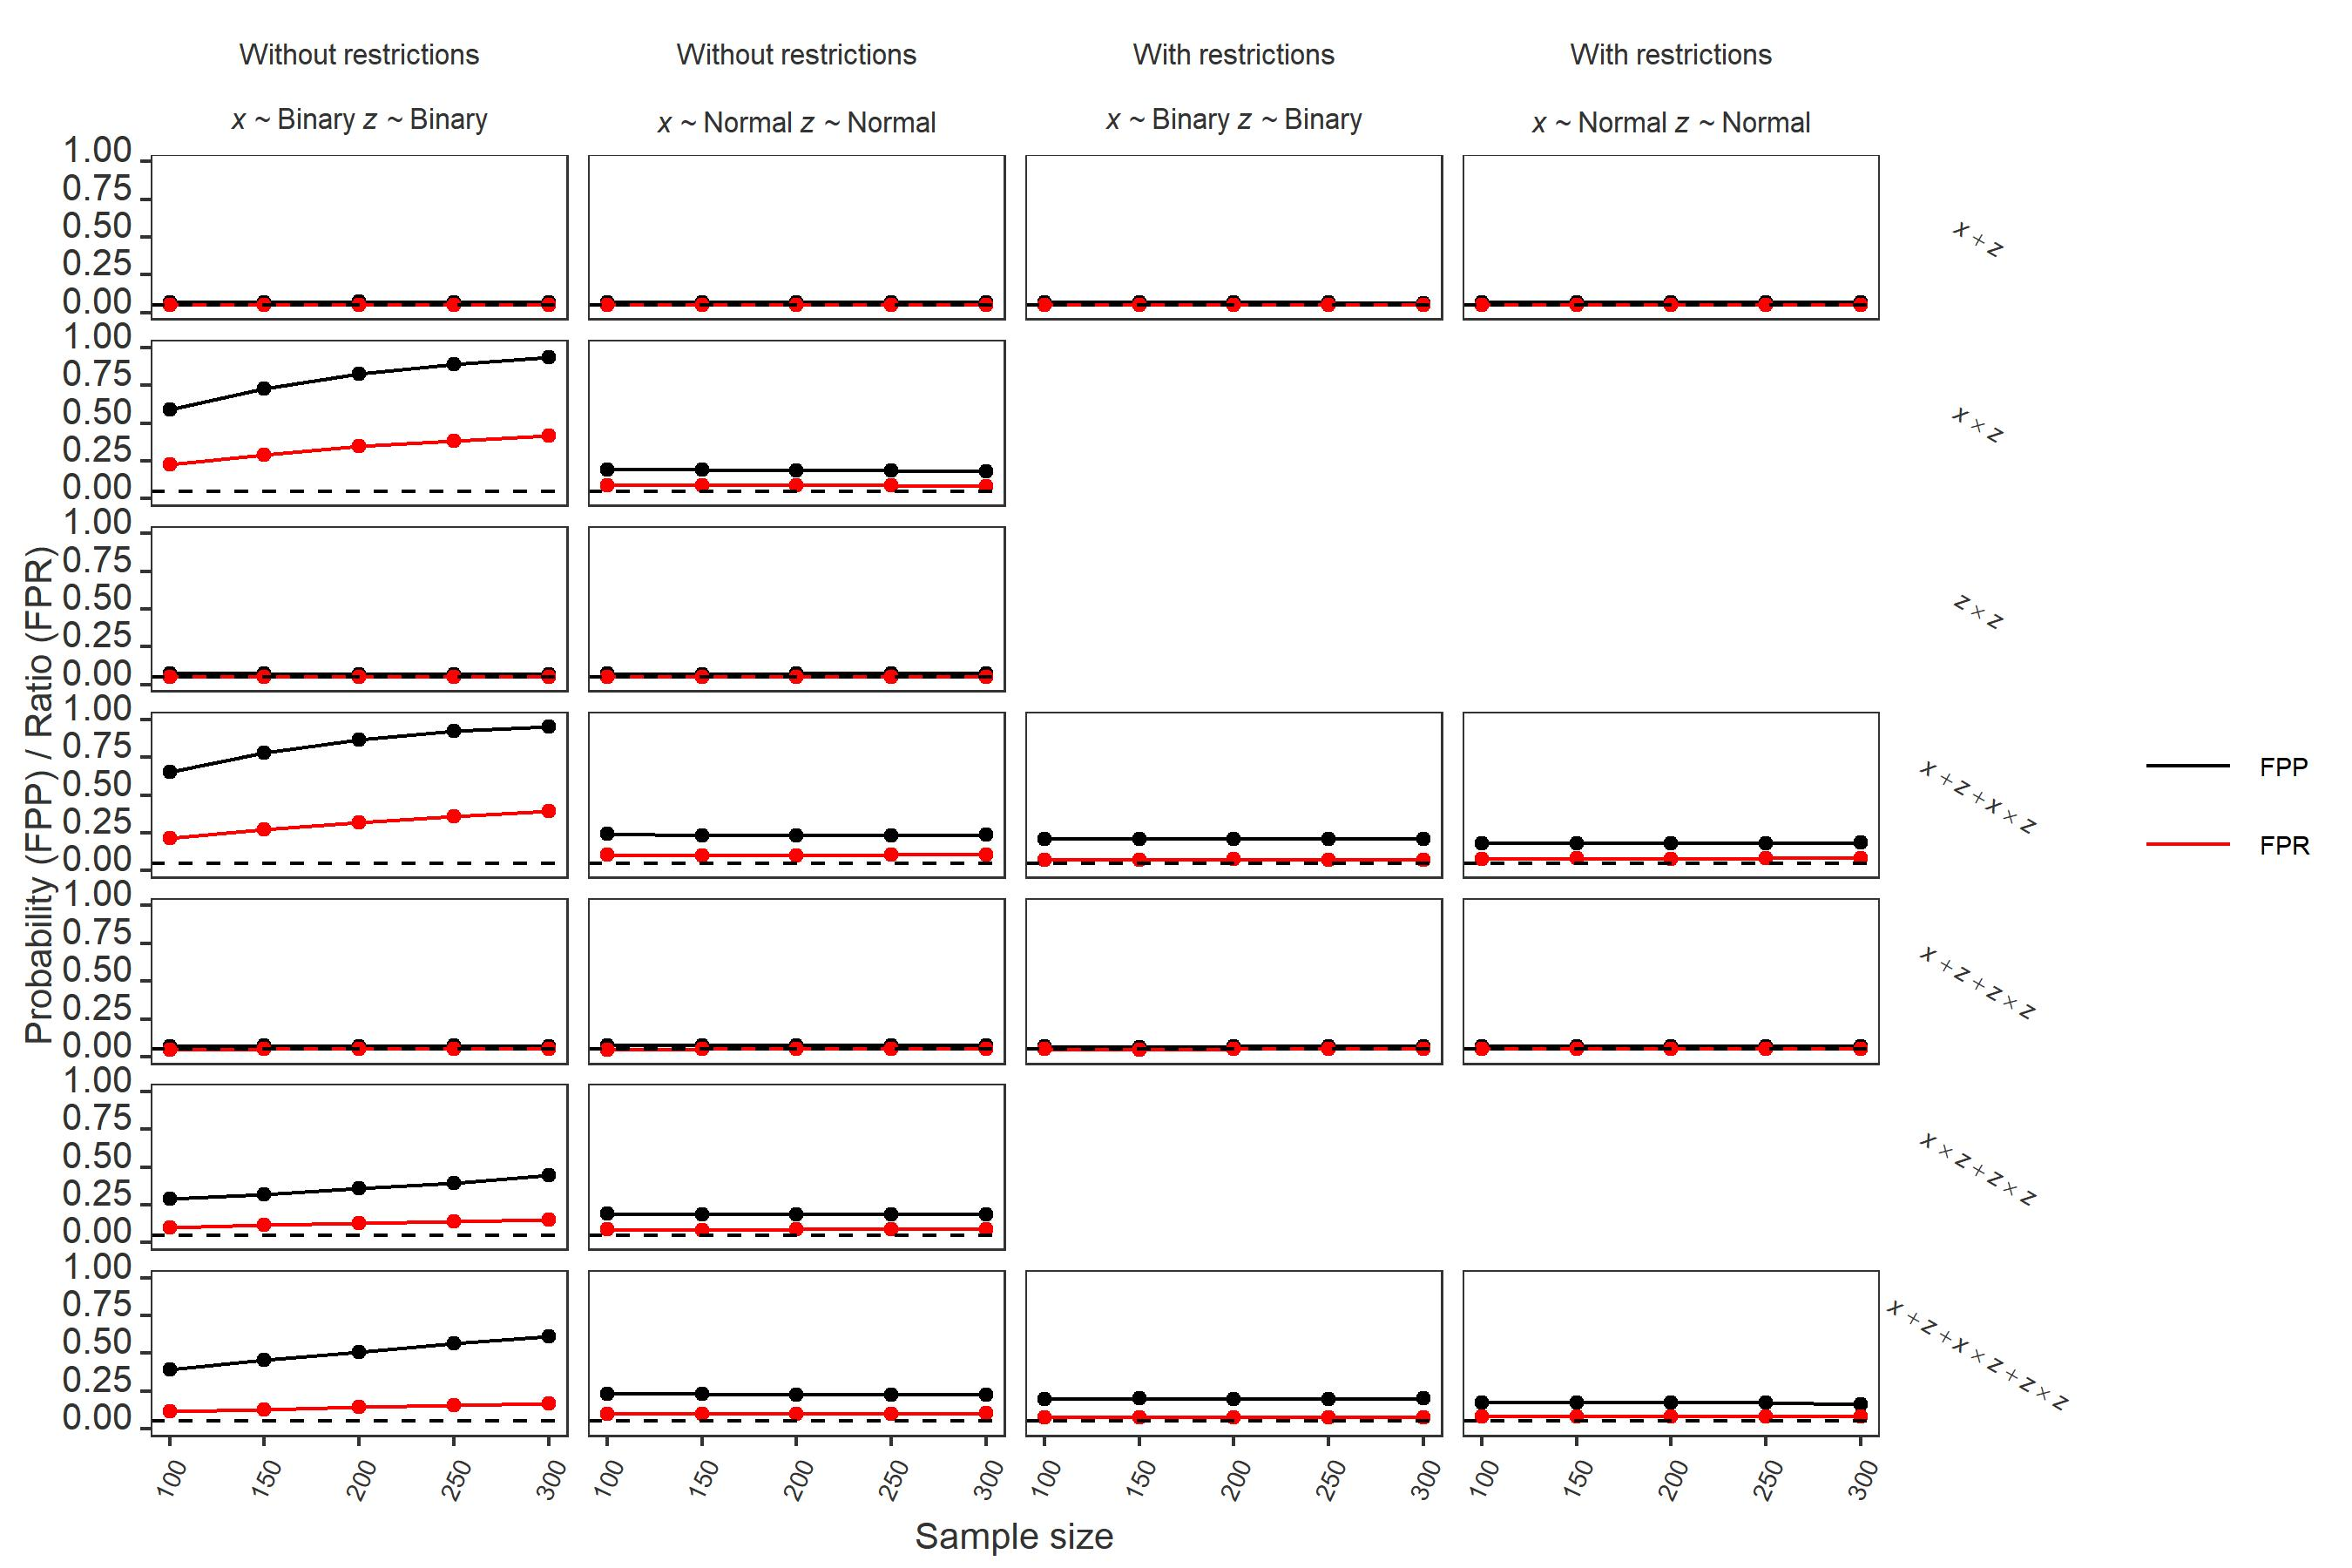
\includegraphics[width=0.9\textwidth]{R/Analysis/Result/Figures/Figure1D.jpeg}
\centering
\caption{The effect of increasing sample size on the false-positive probability and false-positive ratio. Black denotes the false-positive probability and red denotes the false-positive ratio. Dashed blacked line indicates 0.05. The description of the figure is otherwise the same as for Figure \ref{fig:mainfigure1}.}
\label{fig:mainfigure4}
\end{figure}

\subsection{Correlation between dependent variable and covariates}
Increasing the correlation between the dependent variable and the covariates in the baseline model increases the FPP for most conditions and the FPR for some conditions (see Figure \ref{fig:appfigure2}). The model sets with interactions between the variable of interest and covariates have the highest increase in both the FPP and FPR. The effect is most pronounced when the variable of interest and covariates are binary. The increase in the FPP for these sets is as high as 26.5 percentage points when the correlation increases from \textit{r}=0.2 to \textit{r}=0.3. When the correlation increases from \textit{r}=0.3 to \textit{r}=0.4, the FPP increases only in some conditions where the FPP is not already close to 100\%. The increase in correlation also affects the FPR for the same sets increasing it to as much as 14.4\% when going from \textit{r}=0.2 to \textit{r}=0.3 and similar when going from \textit{r}=0.3 to \textit{r}=0.4. 